% soctepmlate
% Author: Vojtěch Boček
% Edit by: Jaroslav Páral
% Version: 2018-02-12
% Source code: https://github.com/RoboticsBrno/soctemplate/
% Base on: http://www.jcmm.cz/cz/sablona-soc.html
% License: CC BY 4.0

\documentclass{template/socthesis}

\usepackage{subcaption}
\usepackage{amsmath}
\usepackage{enumitem}

\addbibresource{text.bib}

\titlecz{Experimentální studium valivých pohybů a~jejich dopadů na~renesančního člověka pohledem Immanuela Kanta}
\titleen{Experimental Study of Rolling Motions and Their Impact on the Renaissance Man from the Perspective of Immaniel Kant}
\author{Jan Novák}
\field{14} % Obory SOČ: 1 - 18 (http://www.soc.cz/obory-soc/)
\school{Gymnázium Brno, třída kpt.~Jaroše}
\mentor{doc. PhDr. Jana Nováková, Ph.D.}
\mentorstatement{doc. PhDr. Jany Novákové, Ph.D.}

% Změňte, pokud se liší
%\region{Jihomoravský}
%\placefooter{Brno 2017}

\begin{document}
	
	\maketitle
	
	\makecopyrightstatement{V~Brně}
	
	\makethanks{Děkuji své školitelce doc. PhDr. Janě Novotné, Ph.D. za obětavou pomoc, podnětné připomínky a nekonečnou trpělivost, kterou mi během práce poskytovala.}
	
	\pagestyle{empty}
	
	\section*{Anotace}
	Cílem této práce je vytvořit univerzální dálkový ovládací pult, který se od běžně dostupných ovladačů liší tím, že umožňuje uživateli rozmístit si libovolně a v~téměř neomezeném množství ovládací prvky ze standardní nabídky modulů.
	
	\subsection*{Klíčová slova}
	univerzální ovladač; řídicí pult; dálkové ovládání; komunikace; modulární konstrukce
	
	\vspace{20mm}
	
	\section*{Annotation}
	The goal of this work is to create a multi-purpose remote control console.
	Unique feature of this console is the possibility for user to place any and almost unlimited amount of operating ele-ments (from range of standard, premade modules) wherever he needs to and in any layout he wants.
	
	\subsection*{Keywords}
	universal controller; control board; remote control; communication; modular construction
	
	\newpage
	\pagestyle{plain}
	
	\tableofcontents % vysází obsah
	
	%%% Začátek práce
	\setcounter{figure}{0}
	\setcounter{table}{0}
	\newpage
	
	%%% Úvod
	\chapter*{Úvod}
\addcontentsline{toc}{chapter}{Úvod} % přidá položku úvod do obsahu

Účelem je stručně a věcně seznámit se záměrem a řešením tématu, důvodem jeho volby, stručně nastínit problém, který má být řešen (a proč); cíl práce (co je předmětem řešení, jakým způsobem se postupuje a k~čemu se má dospět -- co bude výsledkem; cíl práce je „páteří“ práce, je jedním z~kritérií i pro posuzování řešení tématu, zpracování práce); dále v~úvodu uvést, jaký je postup řešení, metody; výzkumná otázka a ústřední hypotéza (obvykle u~empirických výzkumů) -- vše formou charakteristiky záměru tématu a postupu jeho řešení (zdůvodnění), rozpracování je pak v~textu práce.
\newpage
	
	%%% Jak psát
	\chapter{Jak psát}
Abychom mohli napsat odborný text jasně a srozumitelně, musíme splnit několik základních předpokladů\cite{vut-zkousky}:
\begin{itemize}
	\item musíme mít co říci,
	\item musíme vědět, komu to chceme říci,
	\item musíme si dokonale promyslet obsah,
	\item musíme psát strukturovaně.
\end{itemize}

\section{Musíme mít co říci}
Nejdůležitějším předpokladem dobrého odborného textu je myšlenka.
Je-li myšlenka dost závažná, tak přetrvá, i když je neobratně a zmateně podaná.
Chceme-li však myšlenku podat co nejvýstižněji a ušetřit tak čtenáři čas, musíme dodržet určité zásady, o~kterých pojednáme dále.

\section{Musíme vědět, komu to chceme říci}
Dalším důležitým předpokladem dobrého psaní je psát pro někoho.
Píšeme-li si poznámky sami pro sebe, píšeme je jinak než výzkumnou zprávu, článek, diplomovou práci, knihu nebo dopis.
Podle předpokládaného čtenáře se rozhodneme pro způsob psaní, rozsah informace a míru detailů.

\section{Musíme si dokonale promyslet obsah}
Jakmile víme, co chceme říci a komu, musíme si rozvrhnout látku.
Ideální je takové rozvržení, které tvoří logicky přesný a psychologicky stravitelný celek, ve kterém je pro všechno místo a jehož jednotlivé části do sebe přesně zapadají.
Jsou jasné všechny souvislosti a je zřejmé, co kam patří.

Abychom tohoto cíle dosáhli, musíme pečlivě organizovat látku.
Rozhodneme, co budou hlavní kapitoly, co podkapitoly a jaké jsou mezi nimi vztahy.
Diagramem takové organizace je graf, který je velmi podobný stromu, ale ne řetězci.
Při organizaci látky je stejně důležitá otázka, co do osnovy zahrnout, jako otázka, co z~ní vypustit.
Příliš mnoho podrobností může čtenáře právě tak odradit jako žádné detaily.

\section{Musíme začít psát strukturovaně}
Máme-li tedy myšlenku, představu o~budoucím čtenáři, cíl a osnovu textu, můžeme začít psát.
Při psaní prvního konceptu se snažíme zaznamenat všechny své myšlenky a názory vztahující se k~jednotlivým kapitolám a podkapitolám.
Každou myšlenku musíme vysvětlit, popsat a prokázat.
Hlavní myšlenku má vždy vyjadřovat hlavní věta a nikoliv věta vedlejší.

	
	%%% Několik formálních pravidel
	\chapter{Několik formálních pravidel}
Naším cílem je vytvořit jasný a srozumitelný text.
Vyjadřujeme se proto přesně, píšeme dobrou češtinou (nebo zpravidla angličtinou) a dobrým slohem podle obecně přijatých zvyklostí.
Text má upravit čtenáři cestu k~rychlému pochopení problému, předvídat jeho obtíže a předcházet jim.
Dobrý sloh předpokládá \B{bezvadnou gramatiku, správnou interpunkci a vhodnou volbu slov.} Snažíme se, aby náš text nepůsobil příliš jednotvárně používáním malého výběru slov a tím, že některá zvlášť oblíbená slova používáme příliš často.
Pokud používáme cizích slov, je samozřejmým předpokladem, že známe jejich přesný význam.
Ale i českých slov musíme používat ve správném smyslu.
Např.
platí jistá pravidla při používání slova zřejmě.
Je zřejmé opravdu zřejmé? A~přesvědčili jsme se, zda to, co je zřejmé opravdu platí? Pozor bychom si měli dát i na příliš časté používání zvratného se.
Například obratu dokázalo se, že… zásadně nepoužíváme.
Není špatné používat autorského my, tím předpokládáme, že něco řešíme, nebo například zobecňujeme spolu se čtenářem.
V~kvalifikačních pracích použijeme autorského já (například když vymezujeme podíl vlastní práce vůči převzatému textu), ale v~běžném textu se nadměrné používání první osoby jednotného čísla nedoporučuje.

Za pečlivý výběr stojí i \B{symbolika}, kterou používáme ke značení.
Máme tím na mysli volbu zkratek a symbolů používaných například pro vyjádření typů součástek, pro označení hlavních činností programu, pro pojmenování ovládacích kláves na klávesnici, pro pojmenování proměnných v~matematických formulích a podobně.
Výstižné a důsledné značení může čtenáři při četbě textu velmi pomoci.
Je vhodné uvést seznam značení na začátku textu.
Nejen ve značení, ale i v~odkazech a v~celkové tiskové úpravě je důležitá důslednost.

S~tím souvisí i pojem z~typografie nazývaný \B{vyznačování}.
Zde máme na mysli způsob sazby textu pro jeho zvýraznění.
Pro zvolené značení by měl být zvolen i způsob vyznačování v~textu.
Tak například klávesy mohou být umístěny do obdélníčku, identifikátory ze zdrojového textu mohou být vypisovány písmem typu psací stroj.

Uvádíme-li některá fakta, neskrýváme jejich původ a náš vztah k~nim.
Když něco tvrdíme, vždycky výslovně uvedeme, co z~toho bylo dokázáno, co teprve bude dokázáno v~našem textu a co přebíráme z~literatury s~uvedením odkazu na příslušný zdroj.
V~tomto směru nenecháváme čtenáře \B{nikdy na pochybách}, zda jde o~myšlenku naši nebo převzatou z~literatury.

Nikdy neplýtváme čtenářovým časem výkladem triviálních a nepodstatných informací.
Neuvádíme rovněž několikrát totéž jen jinými slovy.
Při pozdějších úpravách textu se nám může některá dříve napsaná pasáž jevit jako zbytečně podrobná, nebo dokonce zcela zbytečná.
Vypuštění takové pasáže nebo alespoň její zestručnění přispěje k~lepší čitelnosti práce! Tento krok ale vyžaduje odvahu zahodit čas, který jsme jejímu vytvoření věnovali.
	
	
	%%% Nikdy to nebude naprosto dokonalé
	\chapter{Nikdy to nebude naprosto dokonalé}
Když jsme už napsali vše, o~čem jsme přemýšleli, uděláme si den nebo dva dny volna a pak si přečteme sami rukopis znovu.
Uděláme ještě poslední úpravy a skončíme.
Jsme si vědomi toho, že \B{vždy zůstane něco nedokončeno}, vždy existuje lepší způsob, jak něco vysvětlit, ale každá etapa úprav musí být konečná.

	
	%%% Typografické a jazykové zásady
	\chapter{Typografické a jazykové zásady}
Při tisku odborného textu typu technická zpráva (anglicky technical report), ke kterému patří například i text kvalifikačních prací, se často volí formát A4 a často se tiskne pouze po jedné straně papíru.
V~takovém případě volte levý okraj všech stránek o~něco větší než pravý – v~tomto místě budou papíry svázány a technologie vazby si tento požadavek vynucuje.
Při vazbě s~pevným hřbetem by se levý okraj měl dělat o~něco širší pro tlusté svazky, protože se stránky budou hůře rozevírat a levý okraj se tak bude oku méně odhalovat.

Horní a spodní okraj volte stejně veliký, případně potištěnou část posuňte mírně nahoru (horní okraj menší než dolní).
Počítejte s~tím, že při vazbě budou okraje mírně oříznuty.

Stupeň písma u~nadpisů různé úrovně volíme podle standardních typografických pravidel.
Pro všechny uvedené druhy nadpisů se obvykle používá polotučné nebo tučné písmo (jednotně buď všude polotučné, nebo všude tučné).
Proklad se volí tak, aby se následující text běžných odstavců sázel pokud možno na pevný rejstřík, to znamená jakoby na linky s~předem definovanou a pevnou roztečí.

Uspořádání jednotlivých částí textu musí být přehledné a logické.
Je třeba odlišit názvy kapitol a podkapitol – píšeme je malými písmeny kromě velkých začátečních písmen.
U~jednotlivých odstavců textu odsazujeme první řádek odstavce asi o~jeden až dva čtverčíky (vždy o~stejnou, předem zvolenou hodnotu), tedy přibližně o~dvě šířky velkého písmene M základního textu.
Poslední řádek předchozího odstavce a první řádek následujícího odstavce se v~takovém případě neoddělují svislou mezerou.
Proklad mezi těmito řádky je stejný jako proklad mezi řádky uvnitř odstavce.

Při vkládání obrázků volte jejich rozměry tak, aby nepřesáhly oblast, do které se tiskne text (tj.
okraje textu ze všech stran).
Pro velké obrázky vyčleňte samostatnou stránku.
Obrázky nebo tabulky o~rozměrech větších než A4 umístěte do písemné zprávy formou skládanky všité do přílohy nebo vložené do záložek na zadní desce.

Obrázky i tabulky musí být pořadově očíslovány.
Číslování se volí buď průběžné v~rámci celého textu, nebo - což bývá praktičtější – průběžné v~rámci kapitoly.
V~druhém případě se číslo tabulky nebo obrázku skládá z~čísla kapitoly a čísla obrázku/tabulky v~rámci kapitoly – čísla jsou oddělena tečkou.
Čísla podkapitol nemají na číslování obrázků a tabulek žádný vliv.

Tabulky a obrázky používají své vlastní, nezávislé číselné řady.
Z~toho vyplývá, že v~odkazech uvnitř textu musíme kromě čísla udat i informaci o~tom, zda se jedná o~obrázek či tabulku (například „… viz tabulka 2.7…“).
Dodržování této zásady je ostatně velmi přirozené.

Pro odkazy na stránky, na čísla kapitol a podkapitol, na čísla obrázků a tabulek a v~dalších podobných příkladech využíváme speciálních prostředků DTP programu, které zajistí vygenerování správného čísla i v~případě, že se text posune díky změnám samotného textu nebo díky úpravě parametrů sazby.

Rovnice, na které se budeme v~textu odvolávat, opatříme pořadovými čísly při pravém okraji příslušného řádku.
Tato pořadová čísla se píší v~kulatých závorkách.
Číslování rovnic může být průběžné v~textu nebo v~jednotlivých kapitolách.
Mezeru neděláme tam, kde se spojují číslice s~písmeny v~jedno slovo nebo v~jeden znak – například 25krát.

Členicí (interpunkční) znaménka tečka, čárka, středník, dvojtečka, otazník a vykřičník, jakož i uzavírací závorky a uvozovky se přimykají k~předcházejícímu slovu bez mezery.
Mezera se dělá až za nimi.
To se ovšem netýká desetinné čárky (nebo desetinné tečky).
Otevírací závorka a přední uvozovky se přimykají k~následujícímu slovu a mezera se vynechává před nimi – (takto) a "takto".

Lomítko se píše bez mezer.
Například školní rok 2013/2014.

\section{Co je to normovaná stránka?}
Pojem normovaná stránka se vztahuje k~posuzování objemu práce, nikoliv k~počtu vytištěných listů.
Z~historického hlediska jde o~počet stránek rukopisu, který se psal psacím strojem na speciální předtištěné formuláře při dodržení průměrné délky řádku 60 znaků a při 30 řádcích na stránku rukopisu.
Vzhledem k~zápisu korekturních značek se používalo řádkování 2 (ob jeden řádek).
Tyto údaje (počet znaků na řádek, počet řádků a proklad mezi nimi) se nijak nevztahují ke konečnému vytištěnému výsledku.
Používají se pouze pro posouzení rozsahu.
Jednou normovanou stránkou se tedy rozumí 60*30 = 1800 znaků.
Obrázky zařazené do textu se započítávají do rozsahu písemné práce odhadem jako množství textu, které by ve výsledném dokumentu potisklo stejně velkou plochu.

Orientační rozsah práce v~normostranách lze v~programu Microsoft Word zjistit pomocí funkce \It{Počet slov} v~menu \It{Nástroje}, když hodnotu \It{Znaky (včetně mezer)} vydělíte konstantou 1800.
Do rozsahu práce se započítává pouze text uvedený v~jádru práce.
Části jako abstrakt, klíčová slova, prohlášení, obsah, literatura nebo přílohy se do rozsahu práce nepočítají.
Je proto nutné nejdříve označit jádro práce a teprve pak si nechat spočítat počet znaků.
Přibližný rozsah obrázků odhadnete ručně.
	
	%%% Slovo Romana
	\chapter{Slovo Romana}
Titulní strana v~takové podobě, v~jaké se vám dostala, je navzdory veškeré projevené snaze velice chatrná a proto vám radím příliš nezasahovat do její stavby, neboť by to mohlo zcela rozhodit pozice všech objektů.
Primární snahou bylo dosáhnout její netečnosti vůči příliš dlouhým jménům (doc.
RNDr.
Jana Šťastně Vdaná, Ph.D.), názvům práce a názvům škol.

I~v~sekci Prohlášení zkuste držet svého kreativního ducha na uzdě, abyste jej vzápětí uplatnili v~celém následujícím textu.
Struktura textu by měla být zhruba následující:

\begin{enumerate}
\item[$\bullet$] úvod
\item teorie
\item metodika
\item výsledky
\item diskuze
\item[$\bullet$] závěr
\end{enumerate}
nicméně není pevně daná a spoustě prací sluší i tematičtější způsoby dělení informací.

\section{Plovoucí objekty}
Všechna čest Microsoftu za postupnou konverzi Wordu z~textového procesoru v~sázecím software.
Jedna z~mnoha vlastností nových verzí je možnost přidání titulku k~plovoucímu objektu, jako bývá obrázek či tabulka.

\begin{figure}[h]
  	\centering
 	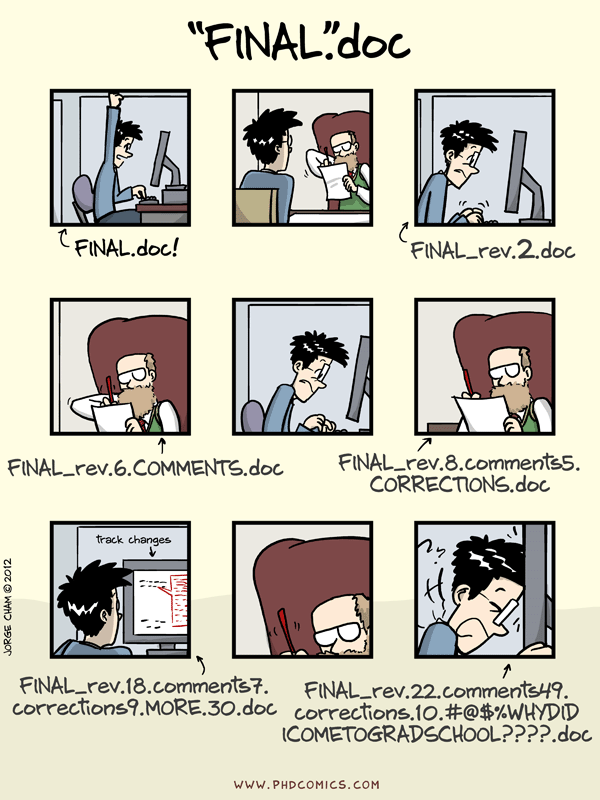
\includegraphics[width=200px]{img/final_doc.png}
 	\caption{Vás to nejspíše čeká taky.}
\end{figure}

\begin{table}[h]
  \centering
    \begin{tabular}{|l|l|}
    \hline
    Jednoduchá & tabulka \\ \hline
    o~& ničem \\
    \hline
    \end{tabular}
  \caption{Jak vidno, čísluje se separátně}
\end{table}

\begin{listedequation}[h]
$$L = - \frac{1}{4}F_{{\mu}v}F^{{\mu}v} + i \overline{\psi} \psi + \psi_i y_i \psi_j \phi + hc + |D_\mu\phi|^2 - V(\phi)$$
\caption{To je ale rovnice!}
\label{eq:hrnekeq}
\end{listedequation}

Vkládání popisků k~obrázkům a tabulkám lze zařídit poměrně snadno a intuitivně tlačítkem „Vložit titulek“ na kartě \It{Reference}.
U~rovnic se bohužel tento způsob uplatňuje jen velmi těžko, klasické vpravo zarovnané (1.1) lze pouze vykouzlit.
(Nápověda Microsoftu radí použít VBA makro, přívrženci Visual Basicu tedy nebudou mít problém.
Obávám se ale, že takových moc nebude.)

Využijte funkci „Vložit seznam obrázků“, která krom seznamu obrázků umí vkládat i seznam tabulek nebo rovnic.
Seznam obrázků v~práci být musí, i kdyby tam byl jen jeden obrázek.
Pro případ nejasnosti upřesňuji, že graf je považován za obrázek.

Co se dá naopak použít skvěle, jsou křížové odkazy.
Klepnutím na tlačítko „Křížový odkaz“ na kartě \It{Reference} mi umožní v~textu odkazovat na právě nějaký z~plovoucích objektů (či kapitolu, sekci, …) Proto nemám potíž zde uvést, že rovnice \autoref{eq:hrnekeq} odpovídá rovnici vyobrazené na hrnku na \autoref{fig:hrnek}, jen s~tím rozdílem, že na hrnku není formulována zcela správně.

\begin{figure}[h]
  	\centering
 	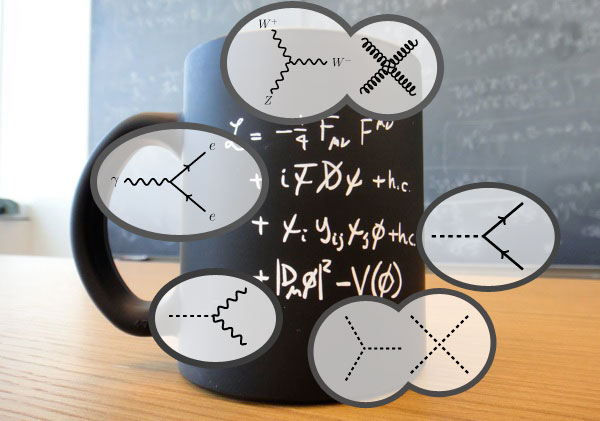
\includegraphics[width=\textwidth]{img/hrnek.jpg}
 	\caption{Hrneček ze Švýcarska}
 	\label{fig:hrnek}
\end{figure}

\section{Bibliografie}
Citovat je důležité (kruciální) a neméně důležité je citovat správně, a to v~ČR podle normy ČSN ISO 690 a ČSN ISO 690-2.
Důvod, proč ji tak mnoho lidí nedělá, je takový: Jedná se o~pěkně otravnou činnost\cite{citovani}.
To se však dá značně eliminovat použitím vhodného softwaru na správu a export citací.
Jaké máme možnosti?

Přímo českou normou se již dlouhou dobu zabývá projekt Citace.com umožňující zdarma získat toliko potřebné bibliografické záznamy.
Proces zkomfortňování šel až tak daleko, že si (např.) čtenáři registrovaní v~Moravské zemské knihovně (do 19 let vč.
zdarma) mohou nainstalovat do svého Wordu doplněk, který téměř vše zařídí za vás.

Pokud náhodou ještě nemáte a nemůžete mít účet v~Moravské zemské knihovně, nemusíte zoufat, i volně přístupná část nástrojů Citací.com má co nabídnout.
Na webu totiž můžete jednoduše vložit ISBN knihy nebo DOI (\It{Digital object identifier}) článku v~časopise a obratem vám bude vygenerována citace přesně podle normy, kterou můžete jednoduše zkopírovat do Wordu.
Číslování v~textu si však budete muset řešit sami.

Nicméně možnosti nekončí Citacemi.com, existuje celá řada dalších nástrojů (třeba EndNote).
Nebojte se požádat o~pomoc své školitele, sami si nejednou prošli stejným problémem a řešení s~velkou pravděpodobností našli.
Tak proč vynalézat kolo?

\subsection{Užitečné odkazy}
\begin{itemize}
    \item \url{http://www.citace.com}, \url{http://www.mzk.cz/}
	\item \url{http://www.boldis.cz/citace/citace1.pdf}
	\item \url{http://www.boldis.cz/citace/citace2.pdf}
	\item \url{https://sites.google.com/site/novaiso690/}
\end{itemize}

\section{Symboly, zkratky, slovníček}
Zkratky vysvětlujeme již při první zmínce v~textu, při jejich častějším výskytu může být praktické uvést ucelený seznam.
Totéž pak platí pro pojmy, které vysvětlujeme v~poznámce pod čarou\footnote{Poznámku pod čarou vložíme opět z~karty \It{Reference} tlačítkem \It{Vložit pozn.
pod čarou.}}: pokud jich je mnoho, vysázíme je i samostatně jako slovníček pojmů.

\section{Moudra závěrem}
Uvědomte si, že hlavním výstupem vaší roční činnosti nejsou data nebo zařízení, nýbrž právě odborný text, který má komisi SOČ ukázat, jak jste studované problematice porozuměli, jaký je váš vlastní přínos, jestli dokážete verbálně vystihnout vše podstatné a důležité.
\It{Formální a estetickou úpravou práce sdělujete komisi, jak moc vám záleží na tom, aby pro ně bylo čtení vaší práce příjemným či alespoň snesitelným zážitkem.}

Šablona je míněna jen jakýmsi odrazovým můstkem a nebojte, pořád na vás zbylo docela dost práce.
Bohužel víc, než jsem původně zamýšlel, protože sázení ve Wordu stále není žádný med a byla by jistě škoda ochudit vás o~četné nadávky na nesmyslnost jeho chování.
Všem počítačově zdatným jedincům pak doporučuji naučit se sazbu v~LaTeXu, je to dovednost, která se vám nikdy neztratí.

\begin{figure}[h]
  	\centering
 	
\includegraphics[width=\textwidth]{img/pulp.jpg}
 	\caption{Nejste v~tom sami.}
\end{figure}

Na závěr vám už poradím jen jedno: hledejte inspiraci.
Velmi dobře si pamatuji ten pocit, kdy sedíte nad prázdným dokumentem a přemýšlíte, co vlastně do té SOČky patří.
Kde začít? Co ještě zmínit a co už raději vynechat? Přitom máme všichni díky theses.cz na dosah stovky tisíc závěrečných prací starších kolegů z~vysokých škol.
Najděte si svůj vzor a jeďte podle něj, odborné posudky vedoucích a oponentů vám dokonce řeknou, co je správně a co nikoliv.

\vspace{\baselineskip}
\noindent Vědě zdar!

\vspace{\baselineskip}
\noindent \B{Roman Beránek} \\
\url{ischemy@gmail.com}

	
	%%% Slovo Jarka
	\chapter{Slovo Jarka}
Trochu bych nesouhlasil s~Romanem ohledně „hlavního výstupu vaší roční činnosti“ a také se zdroji, odkud je vhodné čerpat inspiraci.

Rád bych tato dvě témata na závěr trochu rozebral a zároveň přidal pár slov o~prezentacích, které by měly tvořit podstatnou část vaší práce.

\section{Hlavní výstup vaší roční činnosti}
U~některých oborů možná platí, že hlavním výstupem vaší roční činnosti nejsou data nebo zařízení, nýbrž právě odborný text.
Ovšem z~vlastní zkušenosti mohu říct, že pokud předvedete funkční výtvor (a to ať už softwarový balík pro vývoj a řízení aplikací s~mikročipy, výukový webový portál, univerzální ovládací pult, nebo regulovatelný napájecí zdroj) budete mít na 90 \% větší úspěch než čistě teoretická práce.

Samozřejmě pokud někdo vyvrátí teorii relativity nebo vymyslí novou a lepší periodickou tabulku prvků, bude mít pravděpodobně lepší pozici než vy.
Proto ale musí být vaše práce co možná nejlepší.

Pokud donesete výrobek, který je inovativní, nadčasový, velmi nápaditý a případně vyrobitelný nebo dokonce komerčně prodatelný, a dokážete ho při prezentaci prodat (o~důležitosti prezentace více informací níže), většina porotců vám promine i formální nedostatky a krátký rozsah práce, protože jste jim to předvedli naživo (minimálně toto platí v~rámci oboru strojírenství, elektra a informatiky a podle mě i fyziky, učebních pomůcek atd.)

Kdybych to vzal do extrému, tak práce, která nemá text, ale je velmi zajímavá pro svůj výrobek (zařízení), může klidně vyhrát celostátní kolo SOČ.
Ovšem když přijdu s~textem, kde tento výrobek dokonale popisuji, ale nedovezu, nepředvedu, neukáži, že je funkční, tak jsem na tom hůř než v~prvním případě.

Toto jsou ovšem specifika spíše techničtějších oborů (s~kterými mám zkušenost) a je možné, že v~přírodních vědách (jako chemie, matika, biologie) má spíše Roman pravdu, ale nejsem si tím úplně jistý.
Zvažte sami~:-)

\section{Kde čerpat inspiraci}
Roman jako inspiraci doporučoval theses.cz, ovšem já bych vás spíše odkázal na archiv SOČ (\url{http://soc.nidm.cz/archiv}) a to ze tří důvodů:

\begin{enumerate}[label=\alph*)]
	\item Uvidíte styl a způsob zpracování úspěšných prací SOČ, které vytvořili studenti ve vašem věku a které se porotcům líbily.
	\item Nemusíte se probírat stovkami tisíc závěrečných prací, ale jednoduše si vyberete váš obor a projdete několik nejlepších prací za posledních pár let.
	\item Styl bakalářských a diplomových prací se od SOČek trochu liší a občas je lepší se držet zaběhnutých pravidel SOČ.
\end{enumerate}
Samozřejmě si můžete projít i několik vysokoškolských prací a třeba v~nich najdete i lepší inspiraci.

Jinak nad samostatným formátováním (či některými detaily) neztrácejte mnoho času, protože vám pravděpodobně schází ještě podstatnější věci.
A~také platí, že co porotce/obor, to jiný názor na některé detaily formátování SOČek :-)

\section{Prezentace}
Sebelepší práce bez dobré prezentace je prakticky k~ničemu.
Porotci v~nižších kolech (okresních i krajských) nemají často čas prostudovat si text práce předem.
Tudíž jej občas vidí poprvé, až když danou práci prezentujete.

Pokud budete mít dobrou prezentaci, ve které svoji práci dobře prodáte – ukážete, co jste dělali, jak jste to dělali, co je vaše práce, ale hlavně co je tak unikátního na vaší práci a proč zrovna vy byste měli vyhrát), tak máte z~poloviny vyhráno.
Prezentace tvoří klidně i polovinu hodnocení vaší práce.
Nebo víc.

Proto je podle mě důležité věnovat minimálně stejné množství času přípravě prezentace jako textu.
Pokud postoupíte do dalšího kola, máte většinou možnost si svou práci vzít a do týdne ji upravit/doladit.
Samozřejmě že pokud budete mít perfektní text hned do prvního kola SOČ, budete mít výhodu vůči ostatním a lepší startovací pozici do dalších kol, ale v~případě nedostatku času (což většinou bývá) je vhodnější rozdělit si čas mezi tvorbu textů, prezentace a případně samostatného výrobku.

Samozřejmě se nebojte inspirovat u~svých kolegů z~minulých let například na serveru YouTuBe (hledejte pod „CP SOČ 2013“ a „SOČ 2013 – Brno – krajské kolo“).

O~prezentacích se toho dá samozřejmě napsat mnoho, ale to si necháme třeba na příště ;-)

\vspace{\baselineskip}
\noindent SOČce zdar!

\vspace{\baselineskip}
\noindent \B{Jarek Páral}\\
\url{paral.jarek@gmail.com}
	
	%%% Slovo Lucie
	\chapter{Ještě slovo Lucie}
Pokud si nebudete jistí typografií nebo pravopisem, konzultujte vynikající Internetovou jazykovou příručku.
Píšou ji autoři z~Ústavu pro jazyk český a mezi množstvím balastu na Internetu jí můžete věřit.
Stačí většinou zadat do Google problémové slovo nebo znak spolu s~heslem „ujc“ a víte, na čem jste.

Doufám, že jsme vám pomohli a zpříjemnili práci na vaší SOČce a že shledáte šablonu přínosnou.
Za podněty a reakce budeme všichni tři rádi.

\vspace{\baselineskip}
\noindent Ať to jde!

\vspace{\baselineskip}
\noindent \B{Lucie Vaškeová} \\
\url{lucie.vaskeova@jcmm.cz}
	
	%%% Závěr
	\newpage
\chapter*{Závěr}
\addcontentsline{toc}{section}{Závěr}

Závěrečná kapitola obsahuje zhodnocení dosažených výsledků se zvlášť vyznačeným vlastním přínosem studenta.
Povinně se zde objeví i zhodnocení z~pohledu dalšího vývoje projektu, student uvede náměty vycházející ze zkušeností s~řešeným projektem a uvede rovněž návaznosti na právě dokončené projekty.

	
	\newpage
	\printbibliography[title=Literatura]
	\addcontentsline{toc}{section}{Literatura}
	
	\listoffigures
	\addcontentsline{toc}{section}{Seznam obrázků}
	
	\listoftables
	\addcontentsline{toc}{section}{Seznam tabulek}
	
	\listoflistedequation
	\addcontentsline{toc}{section}{Seznam rovnic}
	
\end{document}
